%**
%*  @file  data.tex
%*  @brief    DIET User's Manual data chapter file
%*  @author  - Philippe COMBES (Philippe.Combes@ens-lyon.fr)
%*  @section Licence 
%*    |LICENSE|

\chapter{\diet data}
\label{ch:data}

It is important that \diet can manipulate data to optimize copies and
memory allocation, to estimate data transfer and computation time,
etc. Therefore the data must be fully described in terms of their data 
types and various attributes associated with these types.

\section{Data types}
\label{sec:types}

\diet defines a precise set of data types to be used to describe the
arguments of the services (on the server side) and of the problems (on
the client side).

The \diet data types are defined in the file
\texttt{$<$install\_dir$>$/include/DIET\_data.h}. The user will also
find in this file various function prototypes to manipulate all \diet
data types. Please refer to this file for a complete and up-to-date
API description.

To keep \diet type descriptions generic, two main sets are used: base and
composite types.

\subsection{Base types}
\label{ssec:base}

Base types are defined in an enum type \texttt{diet\_base\_type\_t} and have the
following semantics:
\begin{center}
\footnotesize
\begin{tabular}{|l|l|c|}
\hline
\textbf{Type}&\textbf{Description}&\textbf{Size in octets}\\
\hline
\textsf{DIET\_CHAR}     & Character                &  1\\
\textsf{DIET\_SHORT}    & Signed short integer     &  2\\
\textsf{DIET\_INT}      & Signed integer           &  4\\
\textsf{DIET\_LONGINT}  & Long signed integer      &  8\\
\textsf{DIET\_FLOAT}    & Simple precision real    &  4\\
\textsf{DIET\_DOUBLE}   & Double precision real    &  8\\
\hline\hline
\textsf{DIET\_SCOMPLEX} & Simple precision complex &  8\\
\textsf{DIET\_DCOMPLEX} & Double precision complex & 16\\
\hline
\end{tabular}
\end{center}

\begin{itemize}
\item[NB:] \textsf{DIET\_SCOMPLEX} and \textsf{DIET\_DCOMPLEX} are not implemented yet.
\end{itemize}

% \fixme{On met les trucs pas implant\'e ?}

\subsection{Composite types}
\label{ssec:complex}

Composite types are defined in an enum type \texttt{diet\_type\_t}:
\begin{center}
\footnotesize
\begin{tabular}{|l|l|}
\hline
\textbf{Type}&\textbf{Possible base types}\\
\hline
\textsf{DIET\_SCALAR} & all base types\\
\textsf{DIET\_VECTOR} & all base types\\
\textsf{DIET\_MATRIX} & all base types\\
\textsf{DIET\_STRING} & \textsf{DIET\_CHAR}\\
\textsf{DIET\_PARAMSTRING} & \textsf{DIET\_CHAR}\\
\textsf{DIET\_FILE}   & \textsf{DIET\_CHAR}\\
\textsf{DIET\_CONTAINER}   & all base types\\
\hline
\end{tabular}
\end{center}

Each of these types requires specific parameters to completely describe the
data (see Figure \ref{fig:data}).


\subsection{Persistence mode}
\label{ssec:persismode}
Persistence mode is defined in an enum type \texttt{diet\_persistence\_mode\_t}

\begin{center}
\footnotesize
\begin{tabular}{|l|l|}
\hline
\textbf{mode}&\textbf{Description}\\
\hline
\textsf{DIET\_VOLATILE} & not stored\\
\textsf{DIET\_PERSISTENT\_RETURN} & stored on server, movable and copy back to client\\
\textsf{DIET\_PERSISTENT} & stored on server and movable\\
\textsf{DIET\_STICKY} & stored and non movable\\
\hline\hline
\textsf{DIET\_STICKY\_RETURN} & stored, non movable and copy back to client\\
\hline
\end{tabular}
\end{center}

\begin{itemize}
\item[NB:] \textsf{DIET\_STICKY\_RETURN} only works with \dagda.
\end{itemize}


\section{Data description}
\label{sec:datadesc}

Each parameter of a client problem is manipulated by \diet using the following
structure:
{\footnotesize
\begin{verbatim}
typedef struct diet_arg_s diet_arg_t;
struct diet_arg_s{
  diet_data_desc_t desc;
  void            *value;
};
typedef diet_arg_t diet_data_t;
\end{verbatim}
}

The second field is a pointer to the memory zone where the parameter
data are stored. The first one consists of a complete \diet data
description, which is better described by a figure than with C code,
since it can be set and accessed through API functions. Figure
\ref{fig:data} shows the data classification used in \diet. Every
``class'' inherits from the root ``class'' \texttt{data}, and could
also be a parent of more detailed classes of data in future versions
of \diet.

\begin{figure}[hpt]
 \begin{center}
  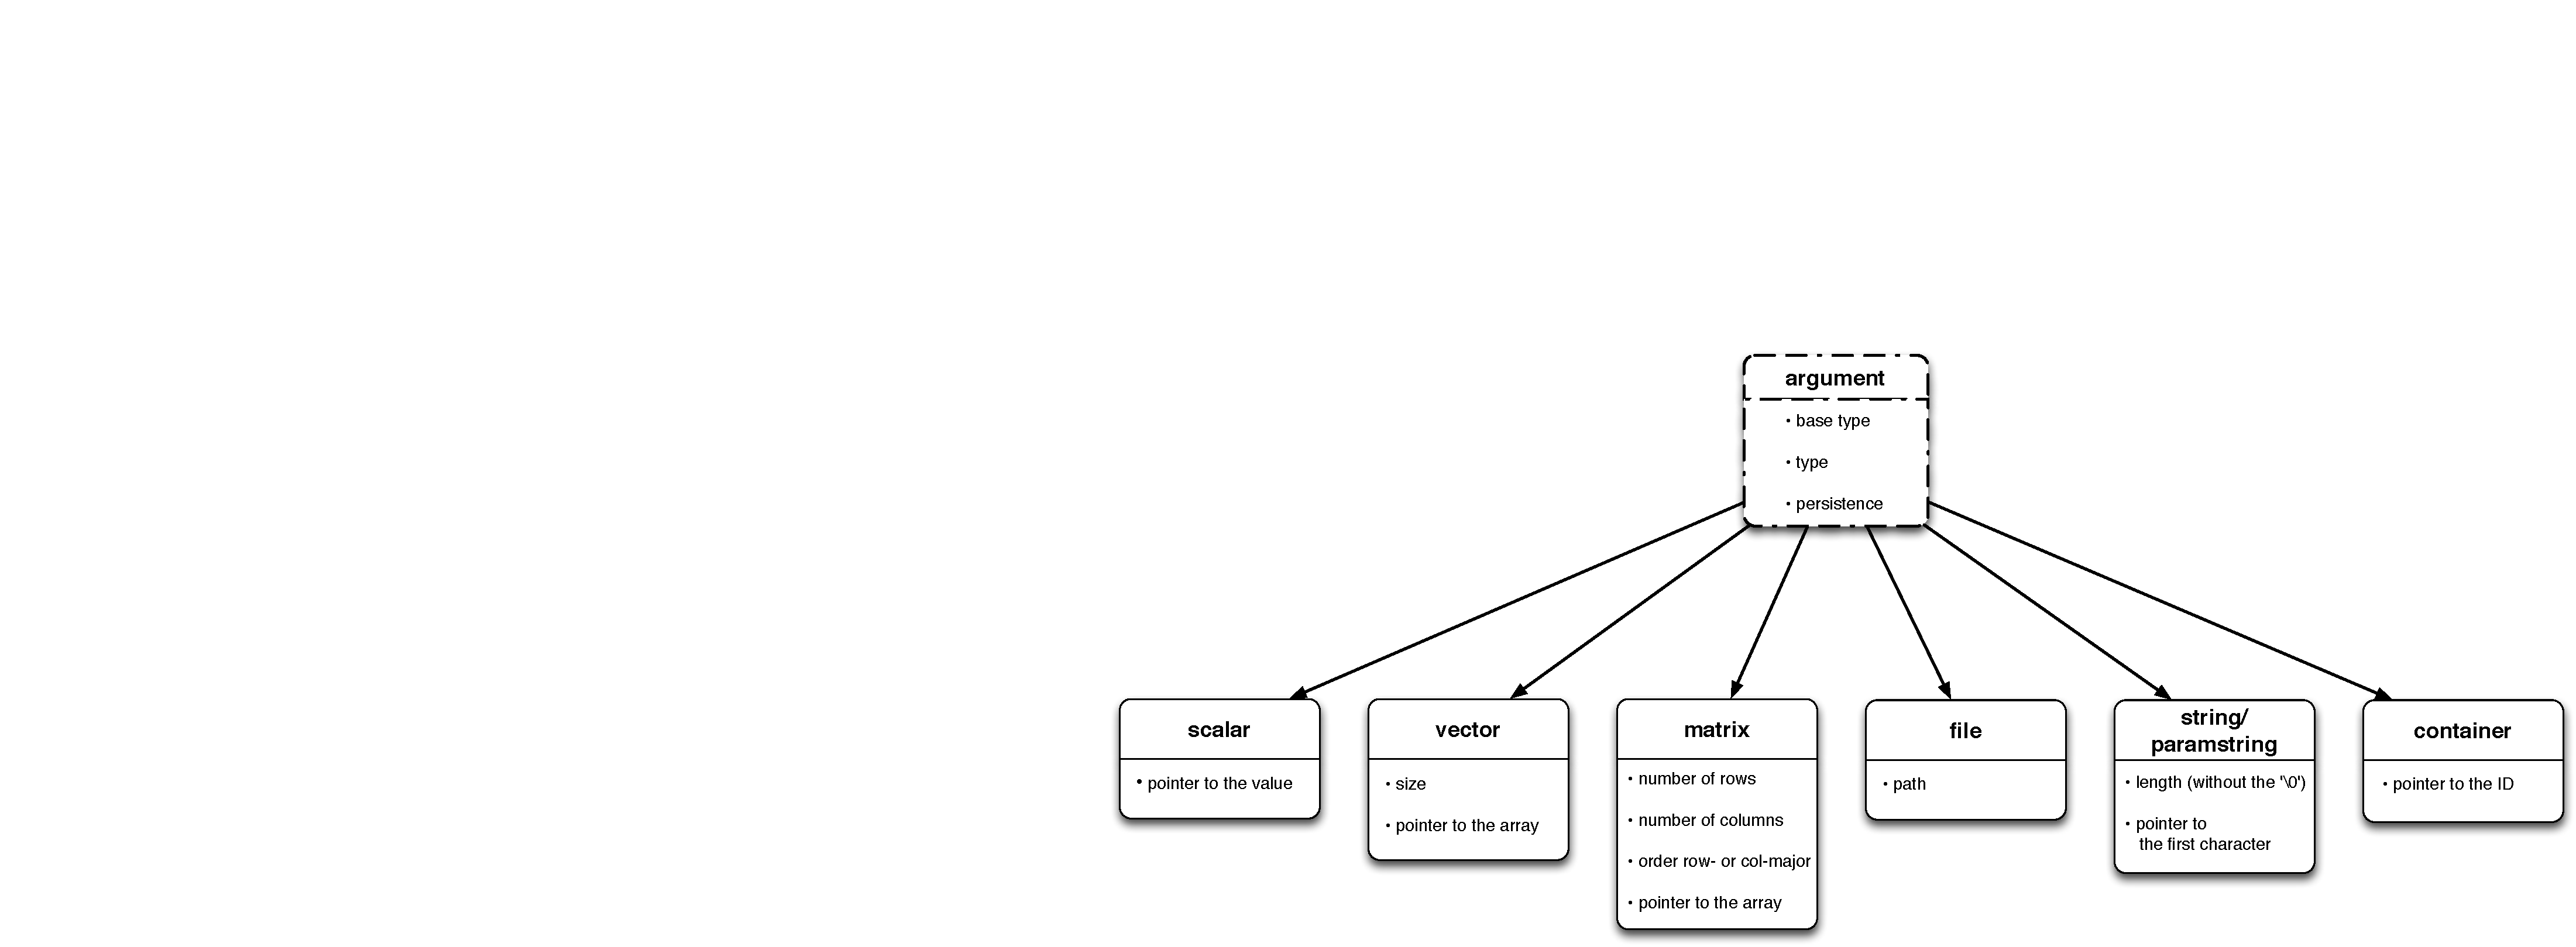
\includegraphics[width=\textwidth]{fig/data}
  \caption{Argument/Data structure description.}
  \label{fig:data}
 \end{center}
\end{figure}


\section{Data management}
\label{sec:datamgt}

\subsection{Data identifier}
\label{ssec:dataid}
The data identifier is generated by the MA. The data identifier is a
string field that contains the MA name, the number of the session plus
the number of the data in the problem (incremental) plus the string
``id''.  This is the \texttt{id} field of the
\texttt{diet\_data\_desc\_t} structure.

{\footnotesize
\begin{verbatim}
typedef struct {
  char* id;  
  diet_persistence_mode_t  mode;
  ....
} diet_data_desc_t;
\end{verbatim}
}

For example, \textbf{id.MA1.1.1} will identify the first data
in the first session submitted on the Master Agent \textbf{MA1}.


\begin{itemize}
\item[NB:] the field ``id'' of the identifier will be next replaced by a
client identifier. This is not implemented yet.
\end{itemize}

\subsection{Data file}
\label{ssec:datafile}

The name of the file is generated by a Master Agent. It is created
during the \texttt{diet\_initialize()} call. The name of the file is
the aggregation of the string ID\_FILE plus the name of the MA plus
the number of the session.  

A file is created only when there are some persistent data in the
session.  

For example, \textbf{ID\_FILE.MA1.1} means the identifiers
of the persistent data stored are in the file corresponding to the
first session in the Master Agent \textbf{MA1}.

The file is stored in the \texttt{/tmp} directory.

% \fixme{Pas configurable ?}

\begin{itemize}
\item[NB:] for the moment, when a data item is erased from the platform, the
file isn't updated.
\end{itemize}


\section{Manipulating \diet structures}
\label{sec:manip}

The user will notice that the API to the \diet data structures consists of
modifier and accessor functions only: no allocation function is required, since
\texttt{diet\_profile\_alloc} (see Section \ref{sec:pbdesc}) allocates all
necessary memory for all argument \textbf{descriptions}. This avoids the
temptation for the user to allocate the memory for these data structures twice
(which would lead to \diet errors while reading profile arguments). Please see
the example in Section \ref{sec:pbex} for a typical example.
\\


Moreover, the user should know that arguments of the \texttt{\_set} functions
that are passed by pointers are \textbf{not} copied, in order to save memory.
This is true for the \emph{value} arguments, but also for the \emph{path} in
\texttt{diet\_file\_set}. Thus, the user keeps ownership of the memory zones
pointed at by these pointers, and he/she must be very careful not to alter it
during a call to \diet.

\subsection{Set functions}

%The data persistence is not available in this current
%version~\footnote{the data persistence will be available in \diet
%  v1.1}, thus fix the mode of the diet persistence parameter to 0.

\label{sec:setfun}
{\footnotesize
\begin{verbatim}
/**
 * On the server side, these functions should not be used on arguments, but only
 * on convertors (see section 5.5).
 * If mode                                is DIET_PERSISTENCE_MODE_COUNT, 
 * or if base_type                        is DIET_BASE_TYPE_COUNT,
 * or if order                            is DIET_MATRIX_ORDER_COUNT,
 * or if size, nb_rows, nb_cols or length is 0,
 * or if path                             is NULL,
 * then the corresponding field is not modified.
 */

int
diet_scalar_set(diet_arg_t* arg, void* value, diet_persistence_mode_t mode,
                diet_base_type_t base_type);
int
diet_vector_set(diet_arg_t* arg, void* value, diet_persistence_mode_t mode,
                diet_base_type_t base_type, size_t size);

/* Matrices can be stored by rows or by columns */
typedef enum {
  DIET_COL_MAJOR = 0,
  DIET_ROW_MAJOR,
  DIET_MATRIX_ORDER_COUNT
} diet_matrix_order_t;

int
diet_matrix_set(diet_arg_t* arg, void* value, diet_persistence_mode_t mode,
                diet_base_type_t base_type,
                size_t nb_rows, size_t nb_cols, diet_matrix_order_t order);
int
diet_string_set(diet_arg_t* arg, char* value, diet_persistence_mode_t mode);

/* The file size is computed and stocked in a field of arg
   ! Warning ! The path is not duplicated !!! */
int
diet_file_set(diet_arg_t* arg, cont char* path, diet_persistence_mode_t mode);
\end{verbatim}
}


\subsection{Access functions}
\label{sec:accessfun}
{\footnotesize
\begin{verbatim}
/**
 * A NULL pointer is not an error (except for arg): it is simply IGNORED.
 * For instance,
 *   diet_scalar_get(arg, &value, NULL),
 * will only set the value to the value field of the (*arg) structure.
 * 
 * NB: these are macros that let the user not worry about casting (int **)
 * or (double **) etc. into (void **).
 */

/**
 * Type: int diet_scalar_get((diet_arg_t *), (void *),
 *                           (diet_persistence_mode_t *))
 */
#define diet_scalar_get(arg, value, mode) \
        _scalar_get(arg, (void *)value, mode)
/**
 * Type: int diet_vector_get((diet_arg_t *), (void **),
 *                           (diet_persistence_mode_t *), (size_t *))
 */
#define diet_vector_get(arg, value, mode, size) \
        _vector_get(arg, (void **)value, mode, size)
/**
 * Type: int diet_matrix_get((diet_arg_t *), (void **),
 *                           (diet_persistence_mode_t *),
 *                           (size_t *), (size_t *), (diet_matrix_order_t *))
 */
#define diet_matrix_get(arg, value, mode, nb_rows, nb_cols, order) \
        _matrix_get(arg, (void **)value, mode, nb_rows, nb_cols, order)
/**
 * Type: int diet_string_get((diet_arg_t *), (char **),
 *                           (diet_persistence_mode_t *))
 */
#define diet_string_get(arg, value, mode) \
        _string_get(arg, (char **)value, mode)
/**
 * Type: int diet_file_get((diet_arg_t *),
 *                         (diet_persistence_mode_t *), (size_t *), (char **))
 */
#define diet_file_get(arg, mode, size, path) \
        _file_get(arg, mode, size, (char **)path)
\end{verbatim}
}


\section{Data Management functions}

\begin{itemize}
\item {The \texttt{store\_id} method} is used to store the
identifier of persistent data. It also accepts a description of
the data stored. This method has to be called after the
\texttt{diet\_call()} so that the identifier exists.
\begin{verbatim}
  store_id(char* argID,char *msg);
\end{verbatim}

\item The \texttt{diet\_use\_data} method allows the client to use a data
item that is already stored in the platform.
\begin{verbatim}
  diet_use_data(diet_arg_t* arg,char* argID);
\end{verbatim}
This function replaces the set functions (see Section \ref{sec:setfun}).

% \fixme{Comment ca se passe, il y avait pas eu une histoire avec la partie
% dagda?}

\begin{itemize}
\item[NB:] a mechanism for data identifier publication hasn't been 
implemented yet. So, exchanges of identifiers between end-users that
want to share data must be done explicitly.
\end{itemize}



\item {The \texttt{diet\_free\_persistent\_data} method} allows the
client to remove a persistent data item from the platform.
\begin{verbatim}
  diet_free_persistent_data(char *argID);
\end{verbatim}

\end{itemize}


{\footnotesize
\begin{verbatim}

/*******************************************************************
 *   Add handler argID and text message msg in the identifier file *
 ******************************************************************/

void 
store_id(char* argID, char* msg);


/** sets only identifier : data is present inside the platform */

void
diet_use_data(diet_arg_t* arg, char* argID);


/******************************************************************
 *  Free persistent data identified by argID                     *
 *****************************************************************/
int
diet_free_persistent_data(char* argID);

\end{verbatim}
}


\subsection{Free functions}
\label{sec:freefun}

The amount of data  pointed at by value fields should be freed through a \diet
API function:
{\footnotesize
\begin{verbatim}
/****************************************************************************/
/* Free the amount of data pointed at by the value field of an argument.    */
/* This should be used ONLY for VOLATILE data,                              */
/*    - on the server for IN arguments that will no longer be used          */
/*    - on the client for OUT arguments, after the problem has been solved, */
/*      when they will no longer be used.                                   */
/* NB: for files, this function removes the file and frees the path (since  */
/*     it has been dynamically allocated by DIET in both cases)             */
/****************************************************************************/

int
diet_free_data(diet_arg_t* arg);
\end{verbatim}
}


\section{Problem description}
\label{sec:pbdesc}

For \diet to match the client problem with a service, servers and clients must
``speak the same language'', \ie they must use the same problem
description. A unified way to describe problems is to use a name and define its
profile with the type \texttt{diet\_profile\_t}:
{\footnotesize
\begin{verbatim}
typedef struct {
  char*       pb_name;
  int         last_in, last_inout, last_out;
  diet_arg_t *parameters;
} diet_profile_t;
\end{verbatim}
}

%%% \fixme{FIXME:
%%% as soon as persistency is integrated, this should become the table Eddy
%%% prepared to explain the transfer policy, depending on the modes.}


The field \emph{parameters} consists of a \texttt{diet\_arg\_t} array of size
$last\_out + 1$. Arguments can be:
\begin{description}
\item{IN:}    The data are sent to the server. The memory is allocated
  by the user.
\item{INOUT:} The data are allocated by the user as for the IN
  arguments, then sent to the server and brought back into the same memory zone
  after the computation has completed, without any copy. Thus freeing this
  memory on the client side while the computation is performed on the
  server would result in a segmentation fault when the data are
  brought back onto the client.
\item{OUT:} The data are created on the server and brought back into a
  newly allocated memory zone on the client. This allocation is performed by
  \diet. After the call has returned, the user can find the result in
  the zone pointed at by the \emph{value} field. Of course, \diet
  cannot guess how long the user will need these data, so the
  user must free the memory him/herself with \texttt{diet\_free\_data}.
\end{description}

%\fixme{This behaviour will be modified soon with the introduction of the
%persistence modes that will let the user leave some data on the
%servers for later computations.}

The fields \emph{last\_in}, \emph{last\_inout} and \emph{last\_out} of the
\texttt{diet\_profile\_t} structure respectively point at the indexes in the
\emph{parameters} array of the last IN, INOUT and OUT arguments. 

Functions to create and destroy such profiles are defined with the prototypes
below: \\
{\footnotesize
\begin{verbatim}
diet_profile_t *diet_profile_alloc(char* pb_name, int last_in, int last_inout, int last_out);
int diet_profile_free(diet_profile_t *profile);
\end{verbatim}
}

The values of \emph{last\_in}, \emph{last\_inout} and \emph{last\_out}
are respectively:
\begin{description}
\item{\emph{last\_in}:} $-1$ + number of input data.

\item{\emph{last\_inout}:} \emph{last\_in} $+$ number of inout data.

\item{\emph{last\_out}:} \emph{last\_inout} $+$ number of out data.
\end{description}

\section{Examples}
\label{sec:pbex}

\subsection{Example 1: without persistency}
Let us consider the product of a scalar by a matrix: the matrix must be
multiplied in-place, and the computation time must be returned.  This
problem has one IN argument (the scalar factor), one INOUT argument (the matrix)
and one OUT argument (the computation time), so its profile will be built as
follows:
\begin{center}
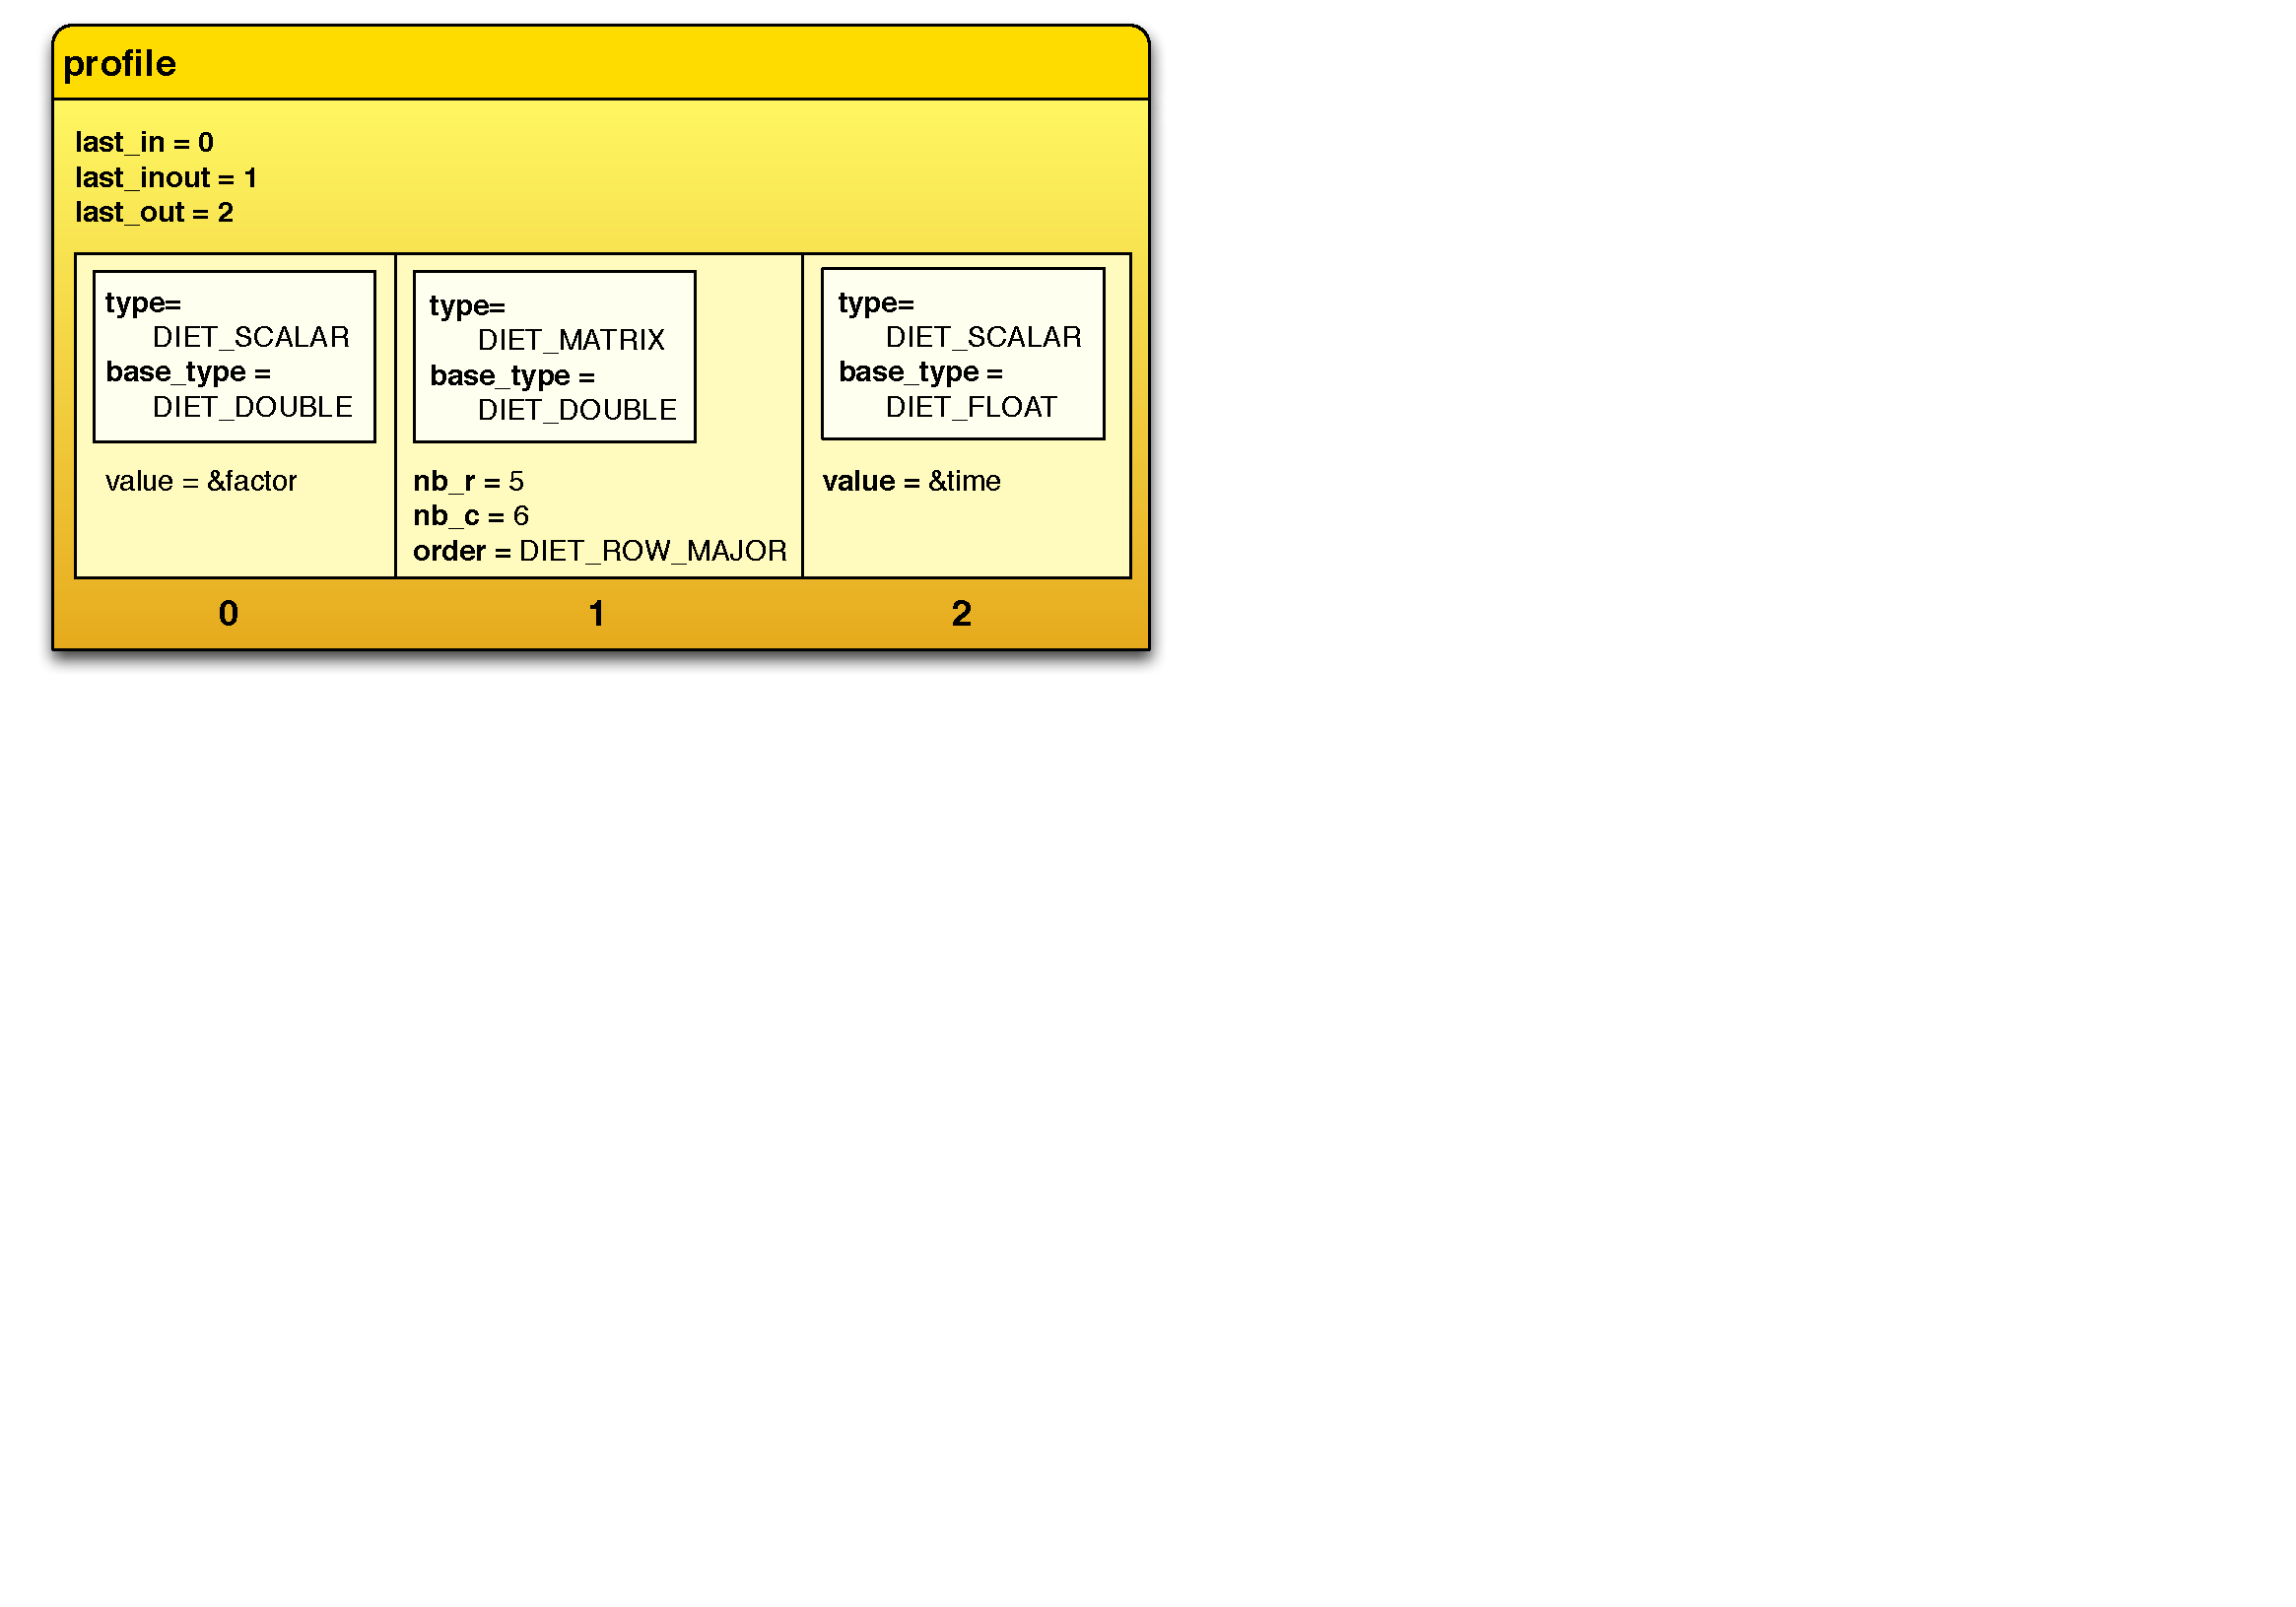
\includegraphics[scale=.55]{fig/smprod}
\end{center}

Here are the lines of C code to generate such a profile:
{\footnotesize
\begin{verbatim}
  double  factor;
  double *matrix;
  float  *time;
  // Init matrix at least, factor and time too would be better ...
  // ...
  diet_profile_t profile = diet_profile_alloc(0, 1, 2); // last_in, last_inout, last_out
  diet_scalar_set(diet_parameter(profile,0), &factor, 0, DIET_DOUBLE);
  diet_matrix_set(diet_parameter(profile,1), matrix,  0, DIET_DOUBLE, 5, 6, DIET_ROW_MAJOR);
  diet_scalar_set(diet_parameter(profile,2), NULL,    0, DIET_FLOAT);
\end{verbatim}
}

\begin{itemize}
\item[NB1:] If there is no IN argument, \emph{last\_in} must be set to
  -1, if there is no INOUT argument, \emph{last\_inout} must
  be equal to \emph{last\_in}, and if there is no OUT argument,
  \emph{last\_out} must be equal to \emph{last\_inout}.
\item[NB2:] The \emph{value} argument for \texttt{\_set} functions
  (\ref{sec:setfun}) is ignored for OUT arguments, since \diet
  allocates the necessary memory space when the corresponding data are
  transferred from the server, so set value to NULL.
\end{itemize}

\subsection{Example 2: using persistency}

Let us consider the following problem : $C=A*B$, with A,B and C
persistent matrices.


{\footnotesize
\begin{verbatim}
  double *A, *B, *C; 
  // matrices initialization
  ...
  diet_initialize();
  strcpy(path,"MatPROD");
  profile = diet_profile_alloc(path, 1, 1, 2);
  diet_matrix_set(diet_parameter(profile,0),
                  A, DIET_PERSISTENT, DIET_DOUBLE, mA, nA, oA);
  print_matrix(A, mA, nA, (oA == DIET_ROW_MAJOR));
  diet_matrix_set(diet_parameter(profile,1),
                  B, DIET_PERSISTENT, DIET_DOUBLE, mB, nB, oB);
  print_matrix(B, mB, nB, (oB == DIET_ROW_MAJOR));
  diet_matrix_set(diet_parameter(profile,2),
                  NULL, DIET_PERSISTENT_RETURN, DIET_DOUBLE, mA, nB, oC);
  
  if (!diet_call(profile)) {
    diet_matrix_get(diet_parameter(profile,2),&C, NULL, &mA, &nB, &oC);
    store_id(profile->parameters[2].desc.id,"matrix C of doubles");
    store_id(profile->parameters[1].desc.id,"matrix B of doubles");
    store_id(profile->parameters[0].desc.id,"matrix A of doubles");
    print_matrix(C, mA, nB, (oC == DIET_ROW_MAJOR));
      
  }
  diet_profile_free(profile);
  // free matrices memory
  ...
  diet_finalize();
\end{verbatim}
}

Then, a client submits the problem : $D=E+C$ with C already present
in the platform. We consider that the handle of C is ``id.MA1.1.3''.

{\footnotesize
\begin{verbatim}
  double *C, *D, *E; 
  // matrices initialization
  ...
  diet_initialize();

  strcpy(path,"MatSUM");
  profile2 = diet_profile_alloc(path, 1, 1, 2);
  
  printf("second pb\n\n");
  diet_use_data(diet_parameter(profile2,0), "id.MA1.1.3");
  diet_matrix_set(diet_parameter(profile2,1),
                  E, DIET_PERSISTENT, DIET_DOUBLE, mA, nB, oE);
  print_matrix(E, mA, nB, (oE == DIET_ROW_MAJOR));
  diet_matrix_set(diet_parameter(profile2,2),
                  NULL, DIET_PERSISTENT_RETURN, DIET_DOUBLE, mA, nB, oD);
  
  if (!diet_call(profile2)) {
   diet_matrix_get(diet_parameter(profile2,2), &D, NULL, &mA, &nB, &oD);
   print_matrix(D, mA, nB, (oD == DIET_ROW_MAJOR));
   store_id(profile2->parameters[2].desc.id,"matrix D of doubles");
   store_id(profile2->parameters[1].desc.id,"matrix E of doubles");
  
  }
  diet_profile_free(profile2);
  diet_free_persistent_data("id.MA1.1.3");
  // free matrices memory
  ...
  diet_finalize();
\end{verbatim}
}  

Note that when a single client creates persistent data with a first
\diet call and uses that data with a second \diet call, we will not
know in advance the identifier of the data.  However, the identifier 
is stored in the structure of the first profile. For example,
consider a matrix A built with
\texttt{diet\_matrix\_set()} method as follows: {\footnotesize
\begin{verbatim}
  ...
  diet_profile_t *profile;
  ...
  diet_matrix_set(diet_parameter(profile,0),
                  E, DIET_PERSISTENT, DIET_DOUBLE, mA, nA, oA);
  ...
\end{verbatim}
} After the first \texttt{diet\_call}, the identifier of A is stored in
the profile \\ (in \texttt{profile->parameters[0].desc.id}). So, for the
second call we will have the following instruction in order to use A:
{\footnotesize
\begin{verbatim}
  ...
  diet_profile_t *profile2;
  ...
  diet_use_data(diet_parameter(profile2,0),profile->parameters[0].desc.id);
  ...
\end{verbatim}
}

\begin{itemize}
\item[NB:] when using this method, the first profile (here
\texttt{profile}) must not be freed before using or making a copy of
the data identifier.
\end{itemize}

% \fixme{Ca marche toujours tout ca?}

%%% Local Variables:
%%% mode: latex
%%% ispell-local-dictionary: "american"
%%% mode: flyspell
%%% fill-column: 79
%%% End:
